\section{Results}
%Explain factually what you found... leave interpretation of what it means for the final discussion section. Here you would include plots of what you found or comparison tables.
For the grapefruit leaves 

%\subsection{Measurements}
% This belongs in results

%\begin{table}
%\caption{Average measured force and area.}
%\label{tbl:results1}
%\begin{center}
%Average force (\si{lbf})\\
%\begin{tabular}{cccc}
%\toprule
%grapefruit & grapefruit & grapefruit & metal leaf \\
%speed 1 & speed 2 & speed 3 & speed 3 \\
%\midrule
%0.051 & 0.061 & 0.79 & 0.014\\
%\bottomrule
%\end{tabular}
%\end{center}
%\begin{center}
%Area data (\si{ft\squared})\\
%\begin{tabular}{cc}
%\toprule
%grapefruit & metal leaf \\
%\midrule
%208 & 32.8 \\
%\bottomrule
%\end{tabular}
%\end{center}
%\end{table}
%


\begin{table}
\caption{Measured raw displacementdata for grapefruit leaf and metal physical model; average force and area. Should be in SI units. Probably would just give a summary table. Was metal leaf displacement really measured in \si{\centi\meter}? Why is metal leaf so small in picture it looks same size. Suggest moving this to appendix and only having a summary in the main text.}
\label{tbl:results1}

\begin{center}
Displacement (\si{in})\\
\begin{tabular}{cccc}
\toprule
grapefruit & grapefruit & grapefruit & metal leaf \\
speed 1 & speed 2 & speed 3 & speed 3(cm) \\ 
\midrule
0.156 & 0.250 & 0.313 & 0.200 \\
0.188 & 0.188 & 0.250 & 0.0500 \\
0.250 & 0.250 & 0.313 & 0.100 \\
0.188 & 0.219 & 0.313 & 0.200 \\
0.188 & 0.250 & 0.313 & 0.150 \\
\bottomrule
\end{tabular}
\end{center}

\begin{center}
Average force (\si{lbf})\\
\begin{tabular}{cccc}
\toprule
grapefruit & grapefruit & grapefruit & metal leaf \\
speed 1 & speed 2 & speed 3 & speed 3 \\
\midrule
0.011 & 0.014 & 0.018 & 0.0032\\
\bottomrule
\end{tabular}
\end{center}

\begin{center}
Area data (\si{ft\squared})\\
\begin{tabular}{cc}
\toprule
grapefruit & metal leaf \\ %& k (lbf/in) \\
\midrule
0.223 & 0.0345 \\ %& 0.059\\
\bottomrule
\end{tabular}
\end{center}
\end{table}



\Fref{fig:results1} shows... (what does it show). When the drag is normalized by area, the effect of leaf flexibility is apparent. \Fref{fig:results2} shows... (what does it show). 

\begin{figure}
\begin{center}
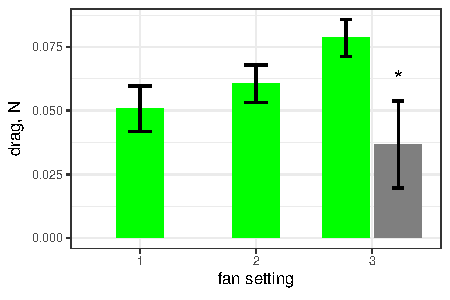
\includegraphics{data/results1.pdf}
\end{center}
\caption{Drag (mean$\pm$sd) for grapefruit (green) and metal (gray) leaves at different fan speeds. The smaller model metal leaf has less drag than the actual grapefruit leaves because of smaller area (two-way ANOVA, $p<\num{1.67e-5}$, $n=5$).}
\label{fig:results1}
\end{figure}

\begin{figure}
\begin{center}
\includegraphics{data/results2.pdf}
\end{center}
\caption{Drag, normalized by area, (mean$\pm$sd) for grapefruit (green) and metal (gray) leaves at different fan speeds. Normalized by area, the rigid metal leaf has significantly more drag than the flexible grapefruit leaves at low speeds and at the highest speed (two-way ANOVA, $p<0.003$, $n=5$).}
\label{fig:results2}
\end{figure}


%\section{Results}
%Explain factually what you found... leave interpretation of what it means for the final discussion section. Here you would include plots of what you found or comparison tables.
% Qualitatively, are there photos showing how the grapefruit leaves moved under wind? Did they bend in particular places, or fold up or rotate in particular ways to reduce their drag?

\begin{table}
\caption{Summary of drag results?}
\begin{center}
\begin{tabular}{ccccc}
      & grapefruit & grapefruit & grapefruit & model \\
      & speed 1 & speed 2 & speed 3 & speed 3 \\
     Average Drag/Area & 0.00024 & 0.00029 & 0.00038 & 0.00045
\end{tabular}
\end{center}
\end{table}

\begin{figure}
    \centering
    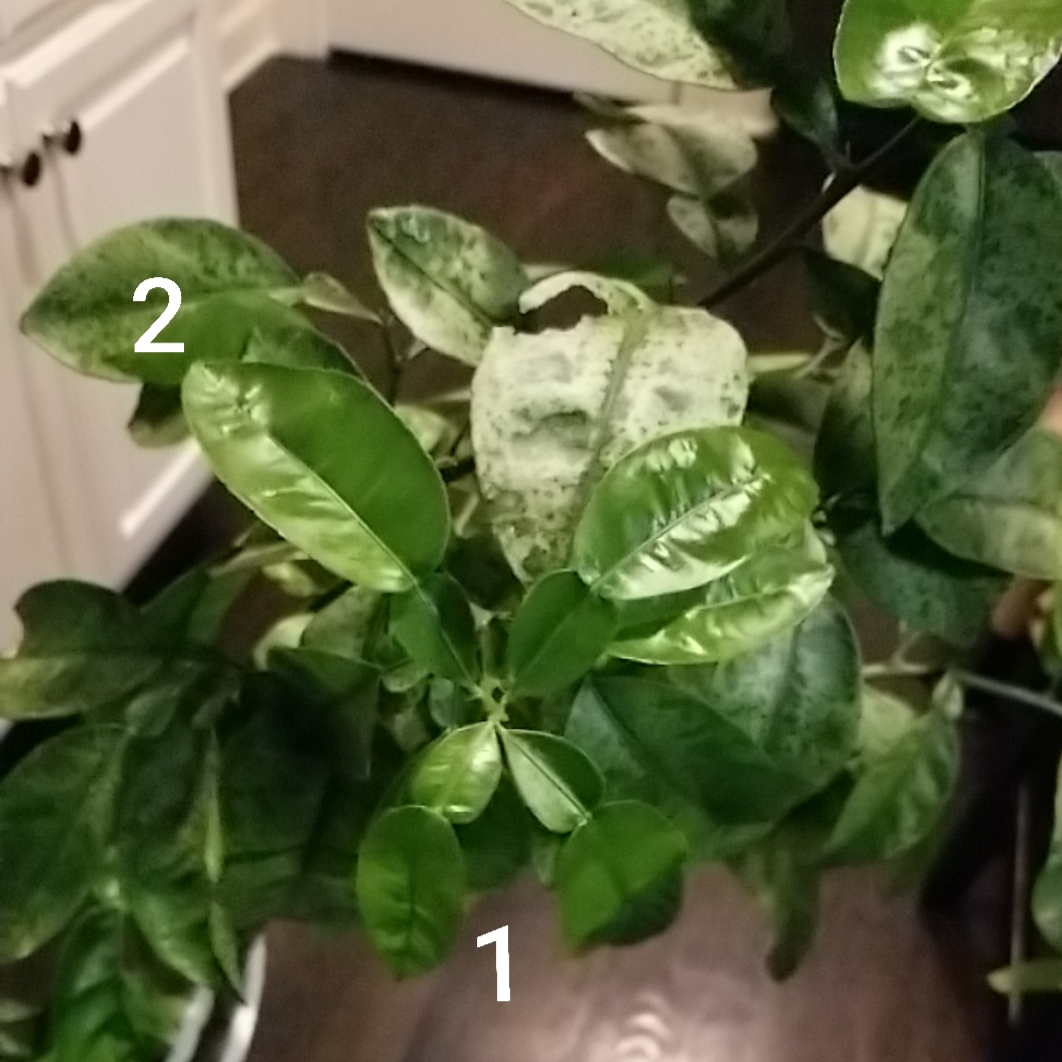
\includegraphics[width=0.49\columnwidth]{figures/Snapshot1.jpg}
    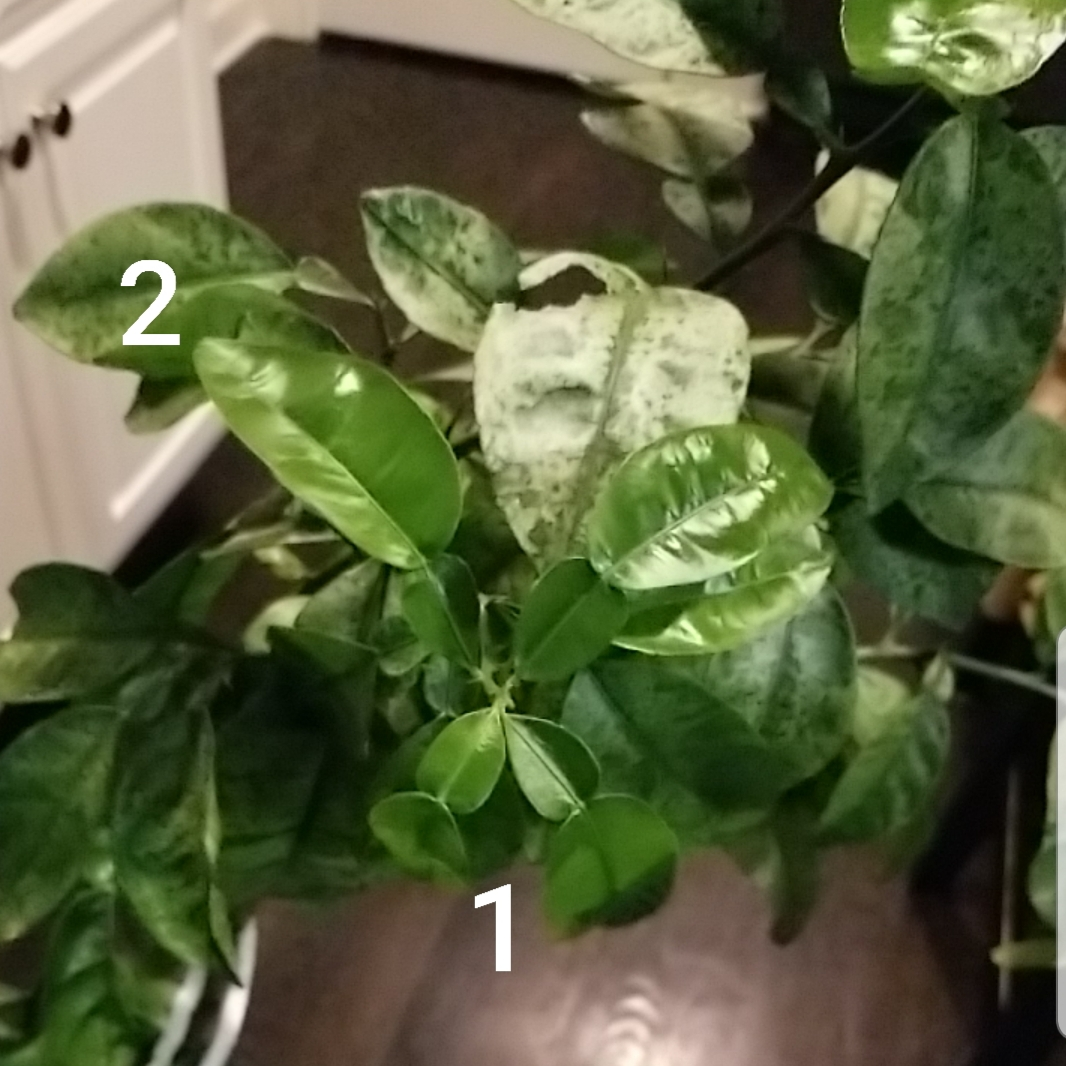
\includegraphics[width=0.49\columnwidth]{figures/Snapshot2.jpg}
    \caption{Caption}
    \label{fig:results1}
\end{figure}

\begin{figure}
    \centering
    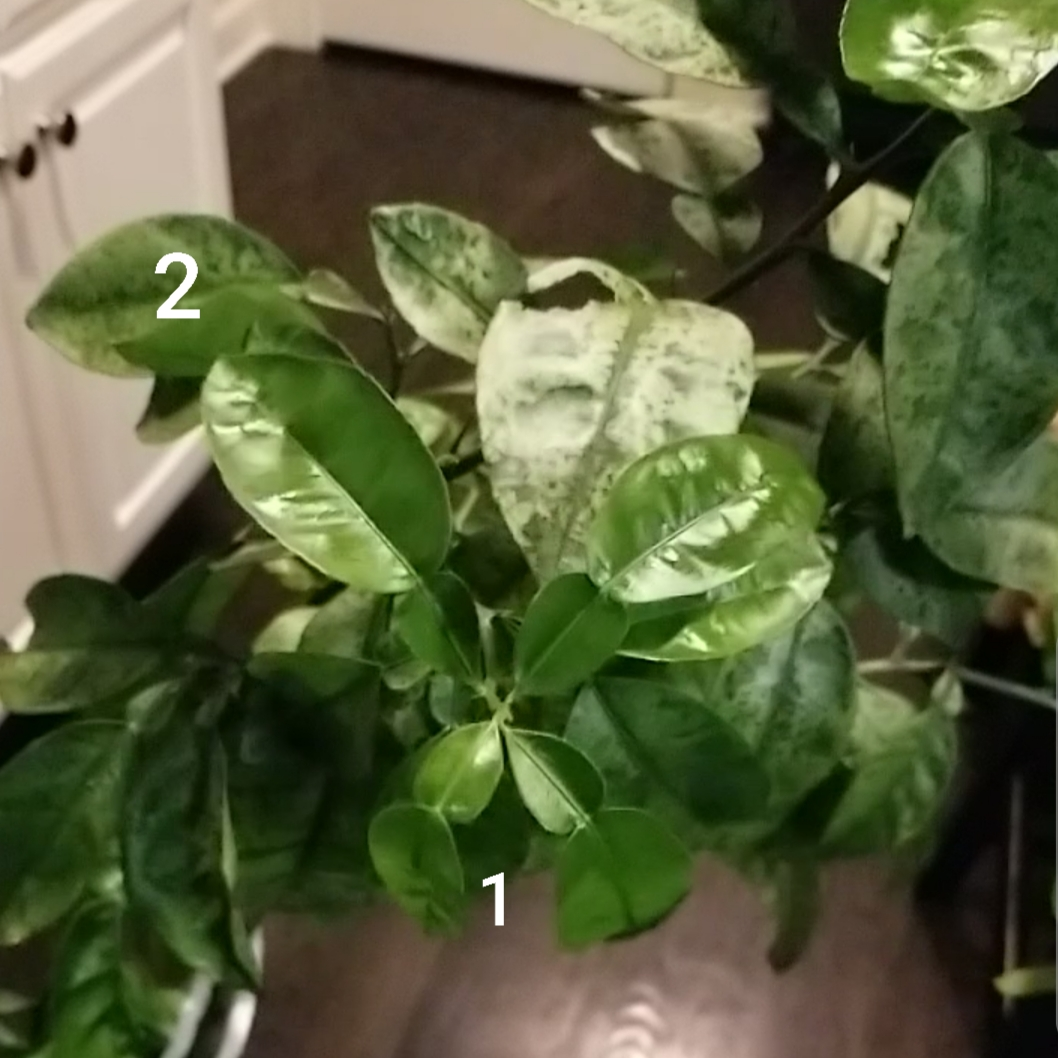
\includegraphics[width=0.49\columnwidth]{figures/Snapshot3.jpg}
    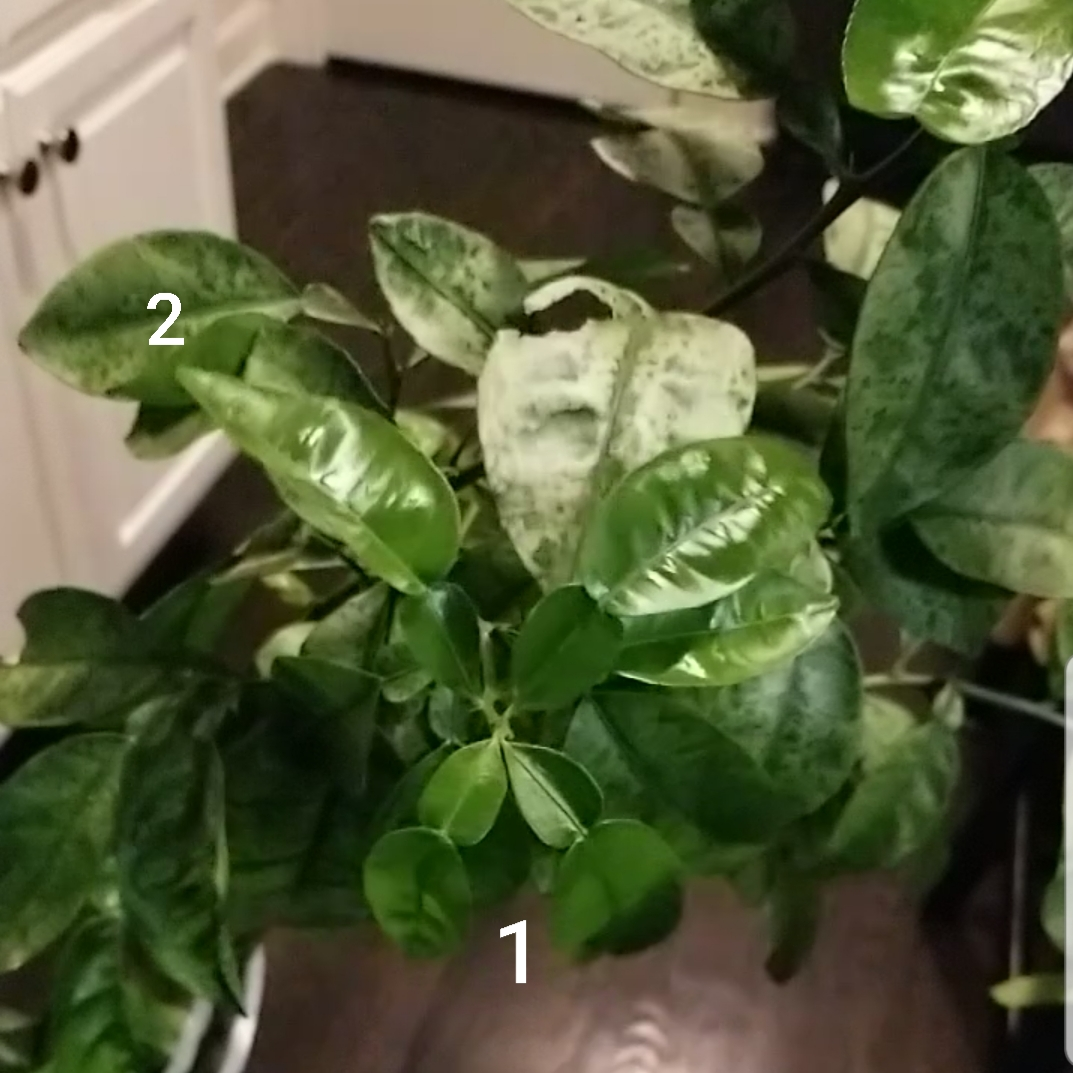
\includegraphics[width=0.49\columnwidth]{figures/Snapshot4.jpg}
    \caption{Caption}
    \label{fig:results2}
\end{figure}

Figures~\ref{fig:results1} and \ref{fig:results2} both show frames from the slow motion video of the \Cxparadisi\ leaves in the wind. Following the leaves indicated by the number 1, the leaves which were struck head-on by the wind flexed quite far at their joints, exposing roughly half of their surface area to the camera. The leaf indicated with the number 2 in \fref{fig:results2} shows the continued vortex shedding on the leaves when wind was blown across them. The leaf pivoted at its joint, but only exposed about half of its area to the wind before returning to its previous state.

\Fref{fig:results3} shows... (what does it show). When the drag is normalized by area, the effect of leaf flexibility is apparent. \Fref{fig:results4} shows... (what does it show). 

\begin{figure}
\begin{center}
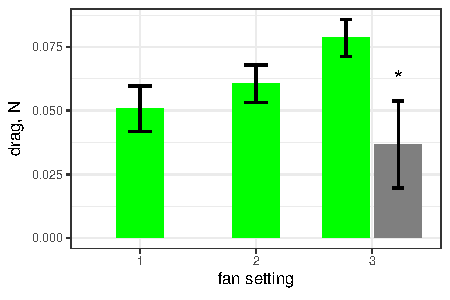
\includegraphics{data/results1.pdf}
\end{center}
\caption{Drag (mean$\pm$sd) for grapefruit (green) and metal (gray) leaves at different fan speeds. The smaller model metal leaf has less drag than the actual grapefruit leaves because of smaller area (two-way ANOVA, $p<\num{1.67e-5}$, $n=5$).}
\label{fig:results3}
\end{figure}

\begin{figure}
\begin{center}
\includegraphics{data/results2.pdf}
\end{center}
\caption{Drag, normalized by area, (mean$\pm$sd) for grapefruit (green) and metal (gray) leaves at different fan speeds. Normalized by area, the rigid metal leaf has significantly more drag than the flexible grapefruit leaves at low speeds and at the highest speed (two-way ANOVA, $p<0.003$, $n=5$).}
\label{fig:results4}
\end{figure}
